% Provenance (never printed): see sources/outline_sources.md (Year 1:
% astronomy of position, spherical trigonometry, time scales, insolation).
% Spherical trigonometry is absent from the mathematics series: this chapter
% owns it. Curves computed in figdata/bachelor-1/{sun_paths, day_length,
% celestial_sphere, spherical_triangle}.py (shared model _solar.py); numbers
% of the exercises and problem in the Book 3 scratch calculator ch01.py.
\chapter{गोलीय खगोल विज्ञान}\label{ch:b1:spherical-astronomy}

किसी कस्बे से दूर एक साफ़ रात में आकाश की ओर इंगित एक दीर्घ-अनावरण कैमरा तारों को
ऐसे वृत्त-चापों के रूप में दर्ज करता है जो सभी एक ही, कभी न हिलने वाले बिंदु के
चारों ओर होते हैं। जो तारा आज रात नौ बजे पूर्व में उगा, वह कल लगभग पाँच मिनट कम नौ
बजे फिर उगेगा, और उसके बाद हर रात थोड़ा पहले। दोपहर को सूर्य जून में दिसंबर की
तुलना में ऊँचा दिखता है, और सुदूर उत्तर में मध्य-ग्रीष्म में वह बिल्कुल अस्त नहीं होता।
यह सब पृथ्वी के अपने अक्ष पर घूमने और सूर्य के चारों ओर उसकी कक्षा का, ज़मीन से
देखा गया रूप है। इसका वर्णन करने के लिए खगोलविद और भूवैज्ञानिक को एक गोले पर
निर्देशांक, उस पर खिंचे त्रिभुजों की त्रिकोणमिति, और ऐसी घड़ियाँ चाहिए जो तारों या सूर्य
के साथ क़दम मिलाकर चलें। यह अध्याय ये औज़ार बनाता है। ये प्लेट गतिकी
(\cref{ch:b1:plate-kinematics}) में लौटते हैं, जहाँ प्लेटें गोले पर घूमती हैं, और जलवायु के
अध्यायों (\cref{ch:b1:radiation-heat-transport}) में, जहाँ किसी \omterm{def:b1:spherical-astronomy:geographic}{अक्षांश} को मिलने वाला
सूर्यप्रकाश पवनों और धाराओं को चलाता है।

\begin{recall}
पृथ्वी एक दिन में एक बार अपने अक्ष पर घूमती है और एक वर्ष में एक बार सूर्य के चारों ओर
एक ऐसी कक्षा पर जाती है जो लगभग वृत्त है; उसका अक्ष कक्षा के सापेक्ष झुका है, और इसी
से ऋतुएँ बनती हैं (भौतिकी की पुस्तकें, कक्षा 6 और 12; केप्लर के नियम भौतिकी की
प्रथम-वर्ष की पुस्तक से स्मरण किए जाते हैं)। पृथ्वी पर किसी बिंदु का स्थान उसके \omterm{def:b1:spherical-astronomy:geographic}{अक्षांश} और
\omterm{def:b1:spherical-astronomy:geographic}{देशांतर} से तय होता है (पुस्तक 1, कक्षा 6)। इकाई लंबाई का सदिश दो कोणों से निश्चित होता है,
जैसे गोलीय निर्देशांकों में; दो इकाई सदिशों का अदिश गुणनफल उनके बीच के कोण की कोज्या है,
और सदिश त्रिक गुणनफल $\vec u\cdot(\vec v\times\vec w)$ तीनों सदिशों के चक्रीय क्रमचय से
अपरिवर्तित रहता है।
\end{recall}

\section{गोलीय त्रिभुज}

\begin{definition}[महावृत्त, गोलीय त्रिभुज]\label{def:b1:spherical-astronomy:spherical-triangle}
गोले का एक \emph{महावृत्त}\index{महावृत्त} उसका वह प्रतिच्छेद है जो उसके केंद्र से होकर
जाने वाले किसी समतल के साथ बनता है; कोई भी दूसरा समतल-काट \emph{लघु वृत्त}\index{लघु वृत्त}
कहलाता है। किन्हीं दो बिंदुओं से, जो व्यासतः विपरीत न हों, ठीक एक महावृत्त गुज़रता है, और
उसके दो चापों में से छोटा चाप गोले पर उन बिंदुओं के बीच सबसे छोटा पथ है। एक
\emph{गोलीय त्रिभुज}\index{गोलीय त्रिभुज} गोले के तीन बिंदुओं से बनी आकृति है, जिसके
शीर्ष $A$, $B$, $C$ हैं और जो \ang{180} से कम के महावृत्त-चापों से जुड़े हैं। उसकी भुजाएँ
$a$, $b$, $c$ ($A$, $B$, $C$ के सम्मुख) केंद्र पर अंतरित कोणों से मापी जाती हैं; उसके कोण
$A$, $B$, $C$ वे कोण हैं जो हर शीर्ष पर मिलने वाली भुजाओं के समतलों के बीच बनते हैं।
\end{definition}

त्रिज्या $R$ वाले गोले पर $a$ रेडियन की एक भुजा की लंबाई $Ra$ है। हर भुजा और हर कोण
$0$ और $\pi$ के बीच होता है।

\begin{omfigure}
\begin{tikzpicture}
\begin{axis}[x=1cm, y=1cm, hide axis, xmin=-2.7, xmax=2.7, ymin=-2.6, ymax=2.6, clip=false]
\draw[black, line width=0.6pt] (axis cs:0,0) circle (2.4cm);
\addplot[black!45, densely dashed, line width=0.4pt] coordinates {(0,0) (-0.078358,1.7847)};
\addplot[black!45, densely dashed, line width=0.4pt] coordinates {(0,0) (-1.5903,-0.2902)};
\addplot[black!45, densely dashed, line width=0.4pt] coordinates {(0,0) (1.4453,-0.16381)};
\addplot[omDef, line width=1.1pt] table {figdata/out/bachelor-1-spherical_triangle-ab.dat};
\addplot[omDef, line width=1.1pt] table {figdata/out/bachelor-1-spherical_triangle-bc.dat};
\addplot[omDef, line width=1.1pt] table {figdata/out/bachelor-1-spherical_triangle-ca.dat};
\addplot[omThm, line width=0.8pt] table {figdata/out/bachelor-1-spherical_triangle-angA.dat};
\addplot[only marks, mark=*, mark size=1.4pt] table[x=x, y=y] {figdata/out/bachelor-1-spherical_triangle-verts.dat};
\fill (axis cs:0,0) circle (1.2pt);
\begin{scope}[font=\small]
  \node[above] at (axis cs:-0.078358,1.7847) {$A$};
  \node[left] at (axis cs:-1.5903,-0.2902) {$B$};
  \node[right] at (axis cs:1.4453,-0.16381) {$C$};
  \node[above left] at (axis cs:0,0) {$O$};
  \node[omThm] at (axis cs:0.24,1.36) {$A$};
  \node[omDef] at (axis cs:0.0,-0.52) {$a$};
  \node[omDef] at (axis cs:0.95,0.95) {$b$};
  \node[omDef] at (axis cs:-1.05,0.95) {$c$};
\end{scope}
\end{axis}
\end{tikzpicture}

{\small गोले पर एक \omterm{def:b1:spherical-astronomy:spherical-triangle}{गोलीय त्रिभुज} $ABC$, जिसका केंद्र $O$ है। भुजाएँ $a$,
$b$, $c$ महावृत्तों के चाप हैं, जिन्हें कोण $BOC$, $COA$, $AOB$ से मापा जाता है; कोण $A$
(लाल) वह कोण है जो $A$ पर मिलने वाली दो भुजाओं के बीच है। बनाए गए त्रिभुज में
$a = \ang{78.6}$, $b = \ang{62.6}$, $c = \ang{64.8}$ हैं और कोण \ang{89.9}, \ang{64.9} और
\ang{67.4} हैं, जिनका योग \ang{180} से अधिक है।}
\end{omfigure}

\begin{theorem}[कोज्या नियम]\label{thm:b1:spherical-astronomy:cosine-rule}
किसी \omterm{def:b1:spherical-astronomy:spherical-triangle}{गोलीय त्रिभुज} में,
\[
  \cos a = \cos b\cos c + \sin b\sin c\cos A .
\]
\end{theorem}

\begin{proof}
इकाई गोले पर काम कीजिए और अक्ष ऐसे चुनिए कि $A$ ध्रुव पर हो:
$\vec A = (0, 0, 1)$, और समतल $xz$ जिसमें $B$ है:
$\vec B = (\sin c, 0, \cos c)$, क्योंकि $B$ की दूरी $c$ है, $A$ से।
बिंदु $C$ की दूरी $b$ है, जो $A$ से नापी जाती है, और वह $A$ से होकर जाने वाले
\omterm{def:b1:spherical-astronomy:spherical-triangle}{महावृत्त} पर है जो कोण $A$ बनाता है, समतल $xz$ के साथ:
$\vec C = (\sin b\cos A, \sin b\sin A, \cos b)$। भुजा $a$, $\vec B$ और $\vec C$ के बीच
का कोण है, इसलिए
\[
  \cos a = \vec B\cdot\vec C = \sin c\sin b\cos A + \cos c\cos b. \qedhere
\]
\end{proof}

\begin{theorem}[ज्या नियम]\label{thm:b1:spherical-astronomy:sine-rule}
किसी \omterm{def:b1:spherical-astronomy:spherical-triangle}{गोलीय त्रिभुज} में,
\[
  \frac{\sin A}{\sin a} = \frac{\sin B}{\sin b} = \frac{\sin C}{\sin c}.
\]
\end{theorem}

\begin{proof}
पिछली उपपत्ति के सदिशों के साथ, उसी तर्क से हम पाते हैं
$\vec B \times \vec C = (-\cos c\sin b\sin A,\ \cos c\sin b\cos A - \sin c\cos b,\
\sin c\sin b\sin A)$, इसलिए त्रिक गुणनफल है
$\vec A\cdot(\vec B\times\vec C) = \sin b\sin c\sin A$। त्रिक गुणनफल $A$, $B$, $C$ के चक्रीय
क्रमचय पर अपरिवर्तित रहता है; $B$, फिर $C$, को ध्रुव पर रखने से उसी तरह $\sin c\sin a\sin B$
और $\sin a\sin b\sin
C$ मिलते हैं। तीनों व्यंजक बराबर हैं; $\sin a\sin b\sin c$ से भाग देने
पर नियम मिल जाता है।
\end{proof}

जब भुजाएँ त्रिज्या की तुलना में छोटी हों, तब $\cos a \approx 1 -
a^2/2$ और $\sin a \approx a$ होता है, और दोनों नियम समतल त्रिभुजों के कोज्या और ज्या नियम
बन जाते हैं: इतने छोटे खंड पर गोला समतल होता है। बड़े त्रिभुज पर ऐसा नहीं होता: \omterm{def:b1:spherical-astronomy:spherical-triangle}{गोलीय
त्रिभुज} के कोणों का योग \ang{180} से अधिक होता है (\cref{exo:b1:spherical-astronomy:12})।

\begin{method}[गोले पर दूरी और दिशा]\label{met:b1:spherical-astronomy:great-circle}
दो स्थानों के, जिनके \omterm{def:b1:spherical-astronomy:geographic}{अक्षांश} $\varphi_1$, $\varphi_2$ और \omterm{def:b1:spherical-astronomy:geographic}{देशांतर} $\lambda_1$, $\lambda_2$ हैं,
बीच की न्यूनतम दूरी और वह दिशा ज्ञात करने के लिए, जिसमें आगे बढ़ना है:
\begin{enumerate}
  \item उत्तरी ध्रुव $P$ और दोनों स्थानों के शीर्षों वाला त्रिभुज बनाइए; ध्रुव से निकलने वाली
        उसकी भुजाएँ \omterm{def:b1:spherical-astronomy:geographic}{सह-अक्षांश} $\ang{90} -
        \varphi_1$ और $\ang{90} - \varphi_2$ हैं, और ध्रुव
        पर उसका कोण \omterm{def:b1:spherical-astronomy:geographic}{देशांतर} का अंतर $\Delta\lambda$ है;
  \item कोज्या नियम कोणीय दूरी $\Delta$ देता है:
        $\cos\Delta = \sin\varphi_1\sin\varphi_2 +
        \cos\varphi_1\cos\varphi_2\cos\Delta\lambda$; दूरी $R\Delta$ है ($\Delta$ रेडियन में);
  \item पहले स्थान पर त्रिभुज का कोण वह है जो उसके सम्मुख भुजा पर कोज्या नियम लगाने से मिलता है:
        $\sin\varphi_2 = \sin\varphi_1\cos\Delta + \cos\varphi_1\sin\Delta\cos
        \mathrm{Az}$, और यह उत्तर से दूसरे स्थान की ओर मापा जाता है।
\end{enumerate}
\omterm{def:b1:spherical-astronomy:spherical-triangle}{महावृत्त} के अनुदिश दिशा बदलती रहती है (किसी याम्योत्तर या विषुवत रेखा के अनुदिश के
अतिरिक्त): जो जहाज़ या विमान एक ही कंपास-दिशा बनाए रखता है, वह एक दूसरे, लंबे वक्र पर चलता है।
\end{method}

\section{खगोलीय निर्देशांक}

\begin{definition}[अक्षांश और देशांतर]\label{def:b1:spherical-astronomy:geographic}
मान लीजिए कि पृथ्वी अपने ध्रुवीय अक्ष पर घूमता हुआ एक गोला है। किसी बिंदु का
\emph{अक्षांश}\index{अक्षांश} $\varphi$ वह कोण है जो विषुवत तल और उस बिंदु से जाने वाली
त्रिज्या के बीच बनता है; यह \ang{-90} (दक्षिण ध्रुव) से \ang{+90} (उत्तर ध्रुव) तक मापा
जाता है। उसका \emph{देशांतर}\index{देशांतर} $\lambda$ वह कोण है जो विषुवत तल में मापा जाता
है और जो बिंदु के याम्योत्तर-अर्धतल तथा एक संदर्भ याम्योत्तर के बीच बनता है, जो ग्रीनविच
से गुज़रता है; यह पूर्व की ओर धनात्मक गिना जाता है, \ang{-180} से \ang{180} तक।
\end{definition}

वास्तव में पृथ्वी थोड़ी चपटी है; मानचित्रों और आकाश के लिए प्रयुक्त \omterm{def:b1:spherical-astronomy:geographic}{अक्षांश} स्थानीय ऊर्ध्वाधर
और विषुवत तल के बीच का कोण है, जो केंद्र से मापे गए कोण से अधिकतम \ang{0.2} भिन्न है
(\cref{ch:b1:isostasy-gravity})। समान \omterm{def:b1:spherical-astronomy:geographic}{अक्षांश} की रेखाएँ, अर्थात् समांतर, \omterm{def:b1:spherical-astronomy:spherical-triangle}{लघु वृत्त} हैं;
याम्योत्तर महावृत्तों के अर्ध-भाग हैं।

\begin{definition}[खगोलीय गोला]\label{def:b1:spherical-astronomy:celestial-sphere}
\emph{खगोलीय गोला}\index{खगोलीय गोला} एक काल्पनिक गोला है जिसका केंद्र प्रेक्षक पर होता है,
और जिस पर हर तारा अपनी दिशा में रखा जाता है; केवल दिशाएँ मायने रखती हैं, दूरियाँ नहीं।
पृथ्वी के अक्ष की बढ़ाइयाँ इसे उत्तरी और दक्षिणी \emph{खगोलीय ध्रुवों}\index{खगोलीय ध्रुव}
पर काटती हैं; पृथ्वी के विषुवत तल का समतल इसे \emph{खगोलीय विषुवत रेखा}\index{खगोलीय विषुवत रेखा} के साथ काटता है। \emph{खमध्य}\index{खमध्य} ठीक ऊपर का बिंदु है, स्थानीय
ऊर्ध्वाधर के अनुदिश; क्षितिज वह \omterm{def:b1:spherical-astronomy:spherical-triangle}{महावृत्त} है जो खमध्य से $\ang{90}$ दूर है।
\emph{स्थानीय याम्योत्तर}\index{स्थानीय याम्योत्तर} वह \omterm{def:b1:spherical-astronomy:spherical-triangle}{महावृत्त} है जो खमध्य और खगोलीय ध्रुवों
से होकर जाता है; वह उत्तर और दक्षिण बिंदुओं पर क्षितिज को काटता है।
\end{definition}

जैसे-जैसे पृथ्वी पश्चिम से पूर्व की ओर घूमती है, \omterm{def:b1:spherical-astronomy:celestial-sphere}{खगोलीय गोला} उलटी दिशा में, अर्थात्
पूर्व से पश्चिम की ओर, \omterm{def:b1:spherical-astronomy:celestial-sphere}{खगोलीय ध्रुवों} के अक्ष पर घूमता प्रतीत होता है, और एक दिन से
थोड़े कम समय में एक चक्कर लगाता है। तारे अपनी सापेक्ष स्थितियाँ बनाए रखते हैं: वे इतनी
दूर हैं कि सूर्य के चारों ओर एक वर्ष की यात्रा उनकी दिशाओं को एक चाप-सेकंड से कम बदलती
है (\cref{ch:b1:observing-the-sky})।

\begin{definition}[क्षैतिज निर्देशांक]\label{def:b1:spherical-astronomy:horizontal}
किसी तारे का \emph{उन्नतांश}\index{उन्नतांश (तारे का)} $h$ क्षितिज के ऊपर उसका कोण है, जो
\ang{-90} से \ang{90} तक है; उसकी खमध्य-दूरी $z = \ang{90} - h$ है। उसका \emph{दिगंश}\index{दिगंश}
$\mathrm{A}$ वह कोण है, जो क्षितिज के अनुदिश उत्तर बिंदु से तारे के ऊर्ध्वाधर वृत्त के पाद तक
मापा जाता है, जो पूर्व से होकर \ang{0} से \ang{360} तक गिना जाता है।
\end{definition}

क्षैतिज निर्देशांक प्रेक्षक के होते हैं: वे स्थान और समय के साथ बदलते हैं। आकाश के अपने
निर्देशांक उसके घूर्णन के साथ चलते हैं।

\begin{definition}[विषुवतीय निर्देशांक]\label{def:b1:spherical-astronomy:equatorial}
किसी तारे की \emph{क्रांति}\index{क्रांति (खगोलीय)} $\delta$ \omterm{def:b1:spherical-astronomy:celestial-sphere}{खगोलीय विषुवत रेखा} से उसका कोण
है, जो उत्तर की ओर धनात्मक है, \ang{-90} से \ang{90} तक। तारे और \omterm{def:b1:spherical-astronomy:celestial-sphere}{खगोलीय ध्रुवों} से होकर
जाने वाला \omterm{def:b1:spherical-astronomy:spherical-triangle}{महावृत्त} उसका घंटा-वृत्त है। तारे का \emph{घंटा कोण}\index{घंटा कोण}
$H$ वह कोण है जो \omterm{def:b1:spherical-astronomy:celestial-sphere}{खगोलीय ध्रुव} पर \omterm{def:b1:spherical-astronomy:celestial-sphere}{स्थानीय याम्योत्तर} और तारे के घंटा-वृत्त के बीच बनता है,
पश्चिम की ओर गिना जाता है, घंटों में, जहाँ एक घंटा \ang{15} के बराबर है। \emph{ऋजु
आरोहण}\index{ऋजु आरोहण} $\alpha$ \omterm{def:b1:spherical-astronomy:celestial-sphere}{खगोलीय विषुवत रेखा} के अनुदिश आकाश के एक निश्चित बिंदु,
\omterm{def:b1:spherical-astronomy:ecliptic}{वसंत विषुव-बिंदु} (\cref{def:b1:spherical-astronomy:ecliptic}) से तारे के घंटा-वृत्त तक का
कोण है, जो पूर्व की ओर गिना जाता है, वह भी घंटों में।
\end{definition}

\omterm{def:b1:spherical-astronomy:equatorial}{क्रांति} और \omterm{def:b1:spherical-astronomy:equatorial}{ऋजु आरोहण} आकाश में स्थिर रहते हैं, जैसे पृथ्वी पर \omterm{def:b1:spherical-astronomy:geographic}{अक्षांश} और \omterm{def:b1:spherical-astronomy:geographic}{देशांतर}; तारा-सूचियाँ
इन्हें सूचीबद्ध करती हैं। \omterm{def:b1:spherical-astronomy:equatorial}{क्रांति} शब्द यहाँ केवल इसी खगोलीय अर्थ में प्रयुक्त है; भौगोलिक
उत्तर और दिक्सूचक के उत्तर के बीच का कोण सदैव चुंबकीय विचलन
कहलाता है (\cref{ch:b1:field-lab-methods-1})।

\begin{proposition}[विषुवतीय से क्षैतिज निर्देशांक]\label{prop:b1:spherical-astronomy:transform}
\omterm{def:b1:spherical-astronomy:geographic}{अक्षांश} $\varphi$ पर, \omterm{def:b1:spherical-astronomy:equatorial}{क्रांति} $\delta$ और \omterm{def:b1:spherical-astronomy:equatorial}{घंटा कोण} $H$ वाले किसी तारे का \omterm{def:b1:spherical-astronomy:horizontal}{उन्नतांश} और \omterm{def:b1:spherical-astronomy:horizontal}{दिगंश}
नीचे दिए सूत्रों से मिलता है:
\[
  \sin h = \sin\varphi\sin\delta + \cos\varphi\cos\delta\cos H,
  \qquad
  \cos\mathrm{A} = \frac{\sin\delta - \sin\varphi\sin h}{\cos\varphi\cos h},
\]
जहाँ $\mathrm{A}$ का मान तारे के याम्योत्तर के पूर्व होने पर \ang{0} और \ang{180} के बीच
होता है ($\sin H < 0$), और पश्चिम होने पर $\mathrm{A} = \ang{360} - \arccos(\dots)$ होता है।
विशेष रूप से, उत्तरी \omterm{def:b1:spherical-astronomy:celestial-sphere}{खगोलीय ध्रुव} का \omterm{def:b1:spherical-astronomy:horizontal}{उन्नतांश} \omterm{def:b1:spherical-astronomy:geographic}{अक्षांश} के बराबर होता है।
\end{proposition}

\begin{proof}
उत्तरी \omterm{def:b1:spherical-astronomy:celestial-sphere}{खगोलीय ध्रुव} $P$, \omterm{def:b1:spherical-astronomy:celestial-sphere}{खमध्य} $Z$ और तारे $X$ से बने त्रिभुज (खगोलीय, या स्थिति, त्रिभुज)
पर विचार कीजिए। स्थानीय ऊर्ध्वाधर विषुवत तल के साथ कोण $\varphi$ बनाता है, इसलिए $PZ =
\ang{90} - \varphi$; $PX = \ang{90} - \delta$; $ZX = \ang{90} - h$। $P$ पर कोण \omterm{def:b1:spherical-astronomy:equatorial}{घंटा कोण} $H$
है; $Z$ पर कोण उत्तर से मापा गया तारे का \omterm{def:b1:spherical-astronomy:horizontal}{दिगंश} है (याम्योत्तर के पूर्व या पश्चिम)। $ZX$
भुजा पर, जो $P$ के सम्मुख है, कोज्या नियम देता है
$\cos(\ang{90} - h) = \cos(\ang{90} - \varphi)\cos(\ang{90} - \delta) +
\sin(\ang{90} - \varphi)\sin(\ang{90} - \delta)\cos H$, यह पहला सूत्र है।
$PX$ भुजा पर, जो $Z$ के सम्मुख है, कोज्या नियम देता है
$\sin\delta = \sin\varphi\sin h + \cos\varphi\cos h\cos\mathrm{A}$, यह दूसरा। ध्रुव के लिए
$\delta = \ang{90}$ है और पहला सूत्र $\sin h = \sin\varphi$ पढ़ा जाता है।
\end{proof}

\begin{omfigure}
\begin{tikzpicture}
\pic (cs) at (0,0) {celestialsphere=45};
\begin{axis}[x=1cm, y=1cm, hide axis, anchor=origin, at={(0,0)}, xmin=-2.6, xmax=2.6, ymin=-2.4, ymax=2.5, clip=false]
\addplot[omField, line width=1.1pt] table[x=x, y=y] {figdata/out/bachelor-1-celestial_sphere-vertical.dat};
\addplot[black!80, line width=0.9pt, densely dash dot] table[x=x, y=y] {figdata/out/bachelor-1-celestial_sphere-hourcircle.dat};
\addplot[only marks, mark=star, mark size=3pt, mark options={line width=0.8pt}] table[x=x, y=y] {figdata/out/bachelor-1-celestial_sphere-star.dat};
\end{axis}
\begin{scope}[font=\footnotesize]
  \node[above] at (cs-Z) {$Z$};
  \node[above left] at (cs-NCP) {$P$};
  \node[left] at (cs-N) {उ};
  \node[right] at (cs-S) {\omnameCompassS};
  \node[below] at (cs-W) {प};
  \node[below, fill=white, fill opacity=0.8, text opacity=1, inner sep=1pt] at (cs-E) {पू};
  \node[above right] at (0.2262,0.94) {$X$};
  \node[omField] at (0.55,0.2) {$h$};
  \node[omDef, right] at (2.0,-1.25) {विषुवत रेखा};
  \node[left] at (-2.0,-0.3) {क्षितिज};
  \node at (-1.35,0.62) {$\varphi$};
\end{scope}
\draw[black!60, line width=0.4pt] (-1.05,0) arc[start angle=180, end angle=137, radius=1.05cm];
\end{tikzpicture}

{\small \omterm{def:b1:spherical-astronomy:geographic}{अक्षांश} \ang{45} उ पर आकाश, पश्चिम से देखा गया, उत्तर बाईं ओर। उत्तरी \omterm{def:b1:spherical-astronomy:celestial-sphere}{खगोलीय ध्रुव} $P$
उत्तर बिंदु के ऊपर \omterm{def:b1:spherical-astronomy:geographic}{अक्षांश} के बराबर \omterm{def:b1:spherical-astronomy:horizontal}{उन्नतांश} पर है (लाल: \omterm{def:b1:spherical-astronomy:celestial-sphere}{खगोलीय ध्रुवों} का अक्ष); \omterm{def:b1:spherical-astronomy:celestial-sphere}{खगोलीय
विषुवत रेखा} (नीली) पूर्व और पश्चिम बिंदुओं पर क्षितिज को काटती है। \ang{25} \omterm{def:b1:spherical-astronomy:equatorial}{क्रांति} वाला
एक तारा $X$ है, जो याम्योत्तर पार करने के बाद तीन घंटे बीस मिनट पर है, अर्थात् \omterm{def:b1:spherical-astronomy:equatorial}{घंटा कोण}
\ang{50} पर, और उसका \omterm{def:b1:spherical-astronomy:horizontal}{उन्नतांश} $h = \ang{45.3}$ और \omterm{def:b1:spherical-astronomy:horizontal}{दिगंश} \ang{261} है (हरा: उसका ऊर्ध्वाधर
वृत्त, \omterm{def:b1:spherical-astronomy:celestial-sphere}{खमध्य} $Z$ से क्षितिज तक); उसका घंटा-वृत्त (बिंदु-रेखा) ध्रुव से तारे के बीच होकर
विषुवत रेखा तक जाता है। गणना \cref{prop:b1:spherical-astronomy:transform} से की गई है।}
\end{omfigure}

\begin{proposition}[याम्योत्तर-पारण और परिध्रुवीय तारे]\label{prop:b1:spherical-astronomy:culmination}
\omterm{def:b1:spherical-astronomy:geographic}{अक्षांश} $\varphi$ पर \omterm{def:b1:spherical-astronomy:equatorial}{क्रांति} $\delta$ वाला तारा याम्योत्तर को ($H = 0$) \omterm{def:b1:spherical-astronomy:horizontal}{उन्नतांश}
$\ang{90} - |\varphi - \delta|$ पर पार करता है; यदि $\delta < \varphi$ तो \omterm{def:b1:spherical-astronomy:celestial-sphere}{खमध्य} के दक्षिण में,
और यदि $\delta > \varphi$ तो उत्तर में। उत्तरी गोलार्ध ($\varphi > 0$) में वह कभी अस्त नहीं
होता यदि $\delta > \ang{90} - \varphi$ हो, और कभी उदय नहीं होता यदि
$\delta < -(\ang{90} - \varphi)$ हो।
\end{proposition}

\begin{proof}
$H = 0$ के लिए, $\sin h = \sin\varphi\sin\delta + \cos\varphi\cos\delta =
\cos(\varphi - \delta)$, इसलिए $h = \ang{90} - |\varphi - \delta|$। न्यूनतम \omterm{def:b1:spherical-astronomy:horizontal}{उन्नतांश}, $H = \ang{180}$ पर, $\sin h = -\cos(\varphi + \delta)$ को संतुष्ट करता है; यह धनात्मक होता है जब
$\varphi + \delta > \ang{90}$। तारा क्षितिज के नीचे रहता है जब उसका अधिकतम \omterm{def:b1:spherical-astronomy:horizontal}{उन्नतांश} भी
ऋणात्मक हो, $|\varphi - \delta| > \ang{90}$।
\end{proof}

\begin{definition}[परिध्रुवीय तारा]\label{def:b1:spherical-astronomy:circumpolar}
एक \emph{परिध्रुवीय तारा}\index{परिध्रुवीय तारा} वह तारा है जो प्रेक्षक के \omterm{def:b1:spherical-astronomy:geographic}{अक्षांश} पर कभी अस्त
नहीं होता: वह \omterm{def:b1:spherical-astronomy:celestial-sphere}{खगोलीय ध्रुव} के चारों ओर घूमता है, याम्योत्तर को ध्रुव के ऊपर पार करता है
और बारह नाक्षत्र घंटे बाद उसके नीचे।
\end{definition}

\begin{omfigure}
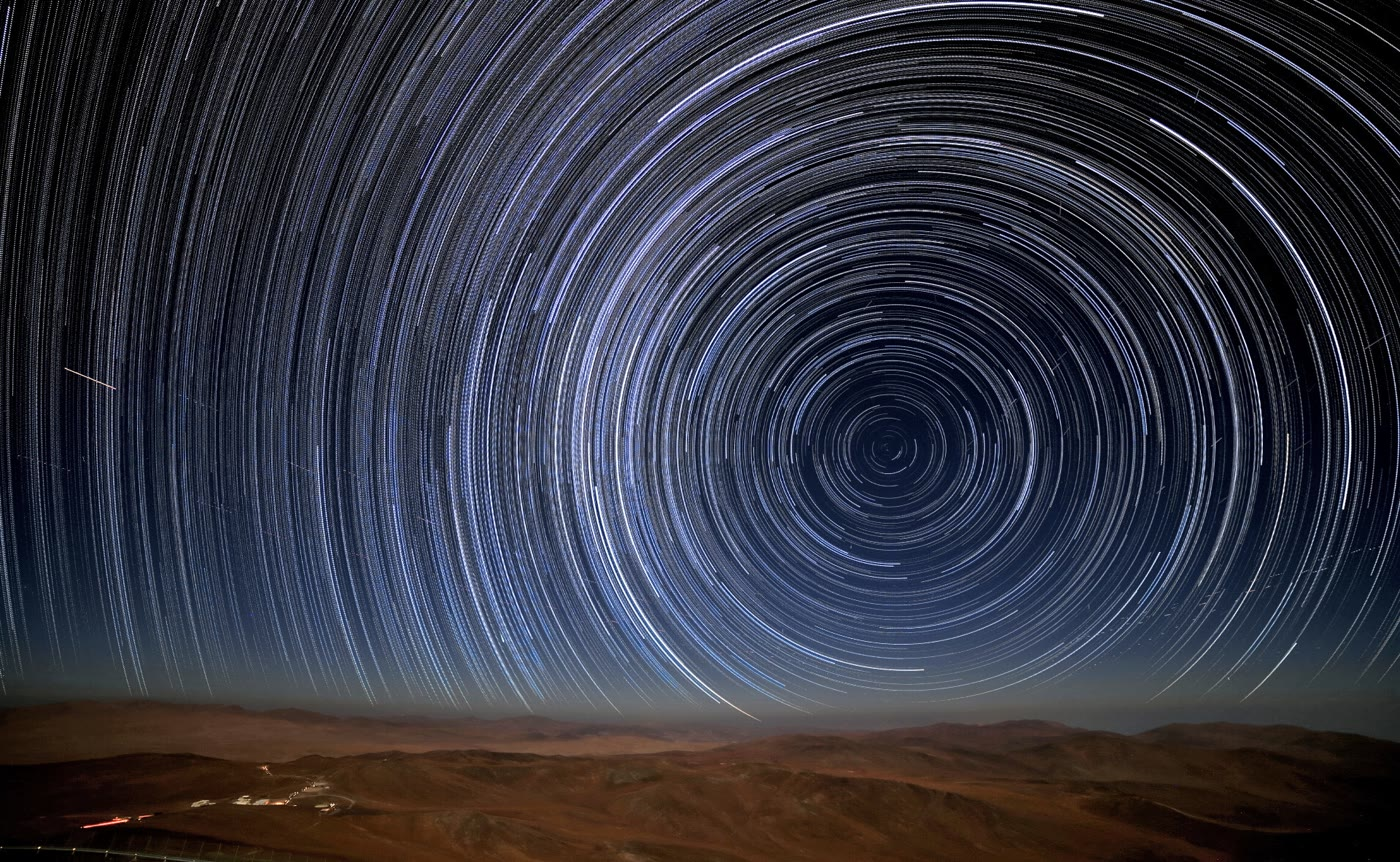
\includegraphics[width=0.8\linewidth]{images/book3/b1-star-trails-paranal.jpg}
% ledger: commons:eso-paranal-star-trails, mpc:paranal

{\small अटाकामा मरुस्थल में पैरानाल वेधशाला के ऊपर तारों के पथ, \omterm{def:b1:spherical-astronomy:geographic}{अक्षांश} \ang{24.6} दक्षिण पर: एक
दीर्घ-अनावरण हर तारे का दक्षिण \omterm{def:b1:spherical-astronomy:celestial-sphere}{खगोलीय ध्रुव} के चारों ओर चाप दर्ज करता है, जो दक्षिणी
क्षितिज से \ang{24.6} ऊपर है। फ़ोटो: वेसन/ESO, CC BY 4.0।}
\end{omfigure}

\section{नाक्षत्र काल और सौर काल}

\begin{definition}[क्रांतिवृत्त]\label{def:b1:spherical-astronomy:ecliptic}
\emph{क्रांतिवृत्त}\index{क्रांतिवृत्त} खगोलीय गोले का वह \omterm{def:b1:spherical-astronomy:spherical-triangle}{महावृत्त} है जिसके अनुदिश सूर्य एक वर्ष में
चलता प्रतीत होता है; वह पृथ्वी की कक्षा के तल का प्रक्षेप है। वह \omterm{def:b1:spherical-astronomy:celestial-sphere}{खगोलीय विषुवत रेखा} से
\emph{क्रांतिवृत्त की तिर्यकता}\index{क्रांतिवृत्त की तिर्यकता} $\varepsilon$ पर झुका है, जो पृथ्वी
के अक्ष का अपनी कक्षा के सापेक्ष झुकाव है। क्रांतिवृत्त विषुवत रेखा को दो बिंदुओं पर काटता है;
\emph{वसंत विषुव-बिंदु}\index{वसंत विषुव-बिंदु} $\gamma$ वह है जहाँ सूर्य मार्च में विषुवत रेखा को
उत्तर की ओर पार करता है। सूर्य का क्रांतिवृत्तीय \omterm{def:b1:spherical-astronomy:geographic}{देशांतर} $\lambda_\odot$ क्रांतिवृत्त के अनुदिश
$\gamma$ से पूर्व की ओर गिना गया उसका कोण है।
\end{definition}

% ledger: earth:obliquity (23.44)
आज तिर्यकता $\varepsilon = \ang{23.44}$ है।

\begin{definition}[नाक्षत्र काल]\label{def:b1:spherical-astronomy:sidereal-time}
स्थानीय \emph{नाक्षत्र काल}\index{नाक्षत्र काल} \omterm{def:b1:spherical-astronomy:ecliptic}{वसंत विषुव-बिंदु} $\gamma$ का \omterm{def:b1:spherical-astronomy:equatorial}{घंटा कोण} है। एक
नाक्षत्र दिवस $\gamma$ के दो बार याम्योत्तर पार करने के बीच का अंतराल है।
\end{definition}

चूँकि \omterm{def:b1:spherical-astronomy:equatorial}{ऋजु आरोहण} $\gamma$ से पूर्व की ओर और \omterm{def:b1:spherical-astronomy:equatorial}{घंटा कोण} याम्योत्तर से पश्चिम की ओर गिना जाता है,
हर तारे के लिए
\[
  H = \mathrm{LST} - \alpha ,
\]
जहाँ LST स्थानीय \omterm{def:b1:spherical-astronomy:sidereal-time}{नाक्षत्र काल} है: कोई तारा तब याम्योत्तर पार करता है जब \omterm{def:b1:spherical-astronomy:sidereal-time}{नाक्षत्र काल} उसके
\omterm{def:b1:spherical-astronomy:equatorial}{ऋजु आरोहण} के बराबर हो। \omterm{def:b1:spherical-astronomy:sidereal-time}{नाक्षत्र काल} दिखाने वाली वेधशाला की घड़ी एक नज़र में बता देती है कि
आकाश का कौन-सा भाग सिर पर है।

\begin{proposition}[नाक्षत्र और सौर दिवस]\label{prop:b1:spherical-astronomy:sidereal-day}
एक \omterm{def:b1:spherical-astronomy:tropical-year}{उष्णकटिबंधीय वर्ष} में, जिसमें $N$ माध्य सौर दिवस हैं, पृथ्वी तारों के सापेक्ष $N + 1$ बार
घूमती है। अतः नाक्षत्र दिवस की अवधि
\[
  \frac{N}{N + 1}\times\qty{24}{h},
\]
होती है, और $N = 365.2422$ पर यह \qty{23}{h}~\qty{56}{min}~\qty{4.09}{s} है: कोई तारा हर दिन
माध्य सौर समय में \qty{3}{min}~\qty{56}{s} पहले याम्योत्तर पार करता है।
\end{proposition}

\begin{proof}
% ledger: usno:tropical-year, earth:Trot (23.9345 h)
तारों और सूर्य के सापेक्ष एक वर्ष में घुमावों की गिनती कीजिए। सूर्य एक वर्ष में \omterm{def:b1:spherical-astronomy:ecliptic}{क्रांतिवृत्त} के
अनुदिश पूर्व की ओर एक बार घूमता है, पृथ्वी के घूर्णन की दिशा में। अतः सूर्य के सापेक्ष पृथ्वी
तारों के सापेक्ष की तुलना में एक घुमाव कम करती है: $N$ सौर दिवस और $N + 1$ नाक्षत्र दिवस एक
ही वर्ष को भरते हैं। नाक्षत्र दिवस एक सौर दिवस का $N/(N+1)$ है, अर्थात्
$\qty{86400}{s}\times 365.2422/366.2422 = \qty{86164.09}{s}$; अंतर $\qty{235.9}{s}$ है। यह
तारों के सापेक्ष पृथ्वी के मापित घूर्णन काल, \qty{23.9345}{h}, से मेल खाता है।
\end{proof}

\begin{definition}[सौर काल]\label{def:b1:spherical-astronomy:solar-time}
\emph{स्पष्ट सौर काल}\index{स्पष्ट सौर काल} सूर्य के \omterm{def:b1:spherical-astronomy:equatorial}{घंटा कोण} के बराबर होता है, जमा 12 घंटे:
धूपघड़ी उसे दिखाती है, और जब सूर्य याम्योत्तर पार करता है तब दोपहर होती है।
\emph{माध्य सौर काल}\index{माध्य सौर काल} एक काल्पनिक माध्य सूर्य का \omterm{def:b1:spherical-astronomy:equatorial}{घंटा कोण} है, जमा 12
घंटे, जो \omterm{def:b1:spherical-astronomy:celestial-sphere}{खगोलीय विषुवत रेखा} के अनुदिश एक समान गति से चलता है और एक \omterm{def:b1:spherical-astronomy:tropical-year}{उष्णकटिबंधीय वर्ष} में एक
चक्कर पूरा करता है। उनका अंतर, स्पष्ट घटा माध्य, \emph{समय का समीकरण}\index{समय का समीकरण}
है।
\end{definition}

वास्तविक सूर्य माध्य सूर्य से दो कारणों से आगे और पीछे चलता है। पृथ्वी उपसौर पर, जनवरी के
आरंभ में, अपसौर की तुलना में तेज़ चलती है, इसलिए \omterm{def:b1:spherical-astronomy:ecliptic}{क्रांतिवृत्त} के अनुदिश सूर्य की प्रगति
असमान है (केप्लर का दूसरा नियम); और सूर्य ऐसे \omterm{def:b1:spherical-astronomy:ecliptic}{क्रांतिवृत्त} पर चलता है जो विषुवत रेखा से झुका
है, इसलिए \omterm{def:b1:spherical-astronomy:ecliptic}{क्रांतिवृत्त} के अनुदिश एक समान गति भी विषुवत रेखा पर, जिसे \omterm{def:b1:spherical-astronomy:equatorial}{घंटा कोण} मापता है,
असमान रूप से प्रक्षिप्त होती है, अयनांतों के पास तेज़ और विषुवों के पास धीमी। घड़ियाँ अपने
समय-क्षेत्र के एक संदर्भ याम्योत्तर पर \omterm{def:b1:spherical-astronomy:solar-time}{माध्य सौर काल} रखती हैं; \omterm{def:b1:spherical-astronomy:geographic}{देशांतर} $\lambda$ पर स्थानीय
माध्य समय ग्रीनविच के समय से $\lambda/\ang{15}$ घंटे आगे है।

\begin{omfigure}
\begin{tikzpicture}
\begin{axis}[omrecord, width=0.9\linewidth, height=5.2cm, xmin=0, xmax=365,
  xtick={0,31,59,90,120,151,181,212,243,273,304,334,365},
  xticklabels={जन,फ़र,मा,अप्र,मई,जून,जुला,अग,सित,अक्तू,नव,दिस,},
  ylabel={समय का समीकरण (मिनट)}, ymin=-20, ymax=21,
  tick label style={font=\scriptsize}, label style={font=\small}]
\addplot[black!50, line width=0.4pt] coordinates {(0,0) (365,0)};
\addplot[omDef, line width=1.1pt] table[x=day, y=eot_min] {figdata/out/bachelor-1-day_length-eot.dat};
\node[font=\scriptsize, above, fill=white, inner sep=1pt] at (axis cs:306,16.6) {$+16.4$};
\node[font=\scriptsize, below, fill=white, inner sep=1pt] at (axis cs:41,-14.4) {$-14.2$};
\end{axis}
\end{tikzpicture}

{\small वर्ष भर का \omterm{def:b1:spherical-astronomy:solar-time}{समय का समीकरण} (स्पष्ट घटा \omterm{def:b1:spherical-astronomy:solar-time}{माध्य सौर काल}): धूपघड़ी नवंबर के आरंभ में
अधिकतम \qty{16.4}{min} आगे और फ़रवरी के मध्य में \qty{14.2}{min} पीछे होती है। गणना 0.0167
उत्केंद्रता, \ang{23.44} तिर्यकता, उपसौर के \omterm{def:b1:spherical-astronomy:geographic}{देशांतर} और 2026 के मार्च विषुव की तिथि वाली
केप्लर कक्षा से की गई है।}
% ledger: earth:ecc, earth:obliquity, nasa:earth-perihelion-longitude, usno:seasons-2026
\end{omfigure}

\section{उदय, अस्त और सूर्य}

\begin{proposition}[उदय और अस्त]\label{prop:b1:spherical-astronomy:rising}
\omterm{def:b1:spherical-astronomy:geographic}{अक्षांश} $\varphi$ पर, \omterm{def:b1:spherical-astronomy:equatorial}{क्रांति} $\delta$ वाला एक तारा जो उगता और अस्त होता है, क्षितिज को घंटा
कोणों $\pm H_0$ पर पार करता है, जहाँ
\[
  \cos H_0 = -\tan\varphi\tan\delta ,
\]
\omterm{def:b1:spherical-astronomy:horizontal}{दिगंश} $\mathrm{A}_0$ पर, जहाँ $\cos\mathrm{A}_0 = \sin\delta/\cos\varphi$ (उदय के समय; वह
$\ang{360} - \mathrm{A}_0$ पर अस्त होता है)। वह $2H_0$ के बराबर अवधि तक क्षितिज के ऊपर रहता है,
जिसे \ang{15} प्रति घंटे पर घंटों में बदला जाता है।
\end{proposition}

\begin{proof}
क्षितिज पर $h = 0$ है, और \cref{prop:b1:spherical-astronomy:transform} देता है
$0 = \sin\varphi\sin\delta + \cos\varphi\cos\delta\cos H_0$, और
$\cos\mathrm{A}_0 = \sin\delta/\cos\varphi$। \omterm{def:b1:spherical-astronomy:equatorial}{घंटा कोण} \ang{15} प्रति घंटे की दर से एक समान
बढ़ता है, उदय पर $-H_0$ से अस्त पर $+H_0$ तक।
\end{proof}

सूर्य के लिए इससे दिन की लंबाई मिलती है, यदि सूर्य को एक बिंदु माना जाए और वायु द्वारा प्रकाश
के मुड़ने की उपेक्षा की जाए (दोनों कुछ मिनट का दिन जोड़ते हैं)। विषुवों पर $\delta = 0$,
$H_0 = \ang{90}$ होता है: हर जगह दिन और रात बारह-बारह घंटे की होती है, और सूर्य ठीक पूर्व में
उगता है।

\begin{omfigure}
\begin{tikzpicture}
\begin{axis}[omrecord, width=0.85\linewidth, height=5.6cm, xmin=40, xmax=320, ymin=0, ymax=75,
  xtick={45,90,135,180,225,270,315}, xticklabels={उपू,पू,दपू,\omnameCompassS,दप,प,उप}, ytick={0,15,30,45,60,75},
  xlabel={दिगंश}, ylabel={सूर्य का उन्नतांश ($^\circ$)},
  tick label style={font=\scriptsize}, label style={font=\small}]
\addplot[omThm, line width=1pt] table[x=az_deg, y=alt_deg] {figdata/out/bachelor-1-sun_paths-june.dat};
\addplot[black, line width=1pt] table[x=az_deg, y=alt_deg] {figdata/out/bachelor-1-sun_paths-equinox.dat};
\addplot[omDef, line width=1pt] table[x=az_deg, y=alt_deg] {figdata/out/bachelor-1-sun_paths-december.dat};
\begin{scope}[font=\scriptsize, fill=white, fill opacity=0.8, text opacity=1, inner sep=1pt]
  \node[omThm, above, fill=white] at (axis cs:180,68.4) {जून अयनांत, $\ang{68.4}$};
  \node[above, fill=white] at (axis cs:180,45) {विषुव, $\ang{45}$};
  \node[omDef, above, fill=white] at (axis cs:180,21.6) {दिसंबर अयनांत, $\ang{21.6}$};
\end{scope}
\end{axis}
\end{tikzpicture}

{\small \ang{45} उत्तरी \omterm{def:b1:spherical-astronomy:geographic}{अक्षांश} पर आकाश में सूर्य का पथ: जून अयनांत पर (लाल), विषुवों पर (काला) और
दिसंबर अयनांत पर (नीला), तथा मध्याह्न के \omterm{def:b1:spherical-astronomy:horizontal}{उन्नतांश} $\ang{90} - \varphi + \delta_\odot$ के साथ।
विषुवों पर सूर्य ठीक पूर्व में उगता और ठीक पश्चिम में अस्त होता है; जून में वह उत्तर-पूर्व में
उगता है।}
\end{omfigure}

\begin{proposition}[सूर्य की क्रांति]\label{prop:b1:spherical-astronomy:sun-declination}
जब सूर्य क्रांतिवृत्तीय \omterm{def:b1:spherical-astronomy:geographic}{देशांतर} $\lambda_\odot$ पर हो, तब उसकी \omterm{def:b1:spherical-astronomy:equatorial}{क्रांति} और \omterm{def:b1:spherical-astronomy:equatorial}{ऋजु आरोहण} संतुष्ट
करते हैं
\[
  \sin\delta_\odot = \sin\varepsilon\sin\lambda_\odot, \qquad
  \tan\alpha_\odot = \cos\varepsilon\tan\lambda_\odot .
\]
\end{proposition}

\begin{proof}
अक्ष ऐसे लीजिए कि $x$ $\gamma$ की ओर हो और $z$ उत्तरी \omterm{def:b1:spherical-astronomy:celestial-sphere}{खगोलीय ध्रुव} की ओर।
\omterm{def:b1:spherical-astronomy:ecliptic}{क्रांतिवृत्त} से जुड़े अक्षों $x$, $y'$, $z'$ में, जिसमें $z'$ उसके ध्रुव की ओर है, सूर्य की दिशा
$(\cos\lambda_\odot, \sin\lambda_\odot, 0)$ है। \omterm{def:b1:spherical-astronomy:ecliptic}{क्रांतिवृत्त} के अक्ष वही हैं जो विषुवत रेखा के
अक्ष, जो कोण $\varepsilon$ से $x$ के परितः घुमाए गए हैं; अतः विषुवतीय अक्षों में सूर्य की दिशा है
$(\cos\lambda_\odot,\ \sin\lambda_\odot\cos\varepsilon,\
\sin\lambda_\odot\sin\varepsilon)$। इसका $z$ घटक $\sin\delta_\odot$ है;
इसके $y$ और $x$ घटकों का अनुपात $\tan\alpha_\odot$ है।
\end{proof}

\begin{omfigure}
\begin{tikzpicture}
\begin{axis}[omrecord, width=0.9\linewidth, height=6cm, xmin=0, xmax=365, ymin=0, ymax=24,
  xtick={0,31,59,90,120,151,181,212,243,273,304,334,365},
  xticklabels={जन,फ़र,मा,अप्र,मई,जून,जुला,अग,सित,अक्तू,नव,दिस,}, ytick={0,6,12,18,24},
  ylabel={दिन की लंबाई (h)}, tick label style={font=\scriptsize}, label style={font=\small},
  legend style={font=\scriptsize, at={(0.5,1.02)}, anchor=south, draw=none}, legend columns=5,
  legend cell align=left]
\addplot[black, line width=0.9pt] table[x=day, y=lat0] {figdata/out/bachelor-1-day_length-lengths.dat};
\addplot[omDef, line width=0.9pt] table[x=day, y=lat30] {figdata/out/bachelor-1-day_length-lengths.dat};
\addplot[omThm, line width=0.9pt] table[x=day, y=lat45] {figdata/out/bachelor-1-day_length-lengths.dat};
\addplot[omField, line width=0.9pt] table[x=day, y=lat60] {figdata/out/bachelor-1-day_length-lengths.dat};
\addplot[black, line width=0.9pt, densely dashed] table[x=day, y=lat70] {figdata/out/bachelor-1-day_length-lengths.dat};
\legend{\ang{0}, \ang{30} उ, \ang{45} उ, \ang{60} उ, \ang{70} उ}
\end{axis}
\end{tikzpicture}

{\small पाँच उत्तरी अक्षांशों पर, वर्ष भर दिन की लंबाई (सूर्य का केंद्र ज्यामितीय क्षितिज के ऊपर),
\cref{prop:b1:spherical-astronomy:rising,prop:b1:spherical-astronomy:sun-declination} से।
\ang{70} उत्तर पर सूर्य जून अयनांत के आसपास हफ़्तों तक ऊपर रहता है और दिसंबर अयनांत के आसपास
नीचे। दक्षिणी गोलार्ध में वक्र आधे वर्ष से खिसके होते हैं।}
\end{omfigure}

\begin{definition}[सूर्यातप]\label{def:b1:spherical-astronomy:insolation}
किसी स्थान और क्षण पर \emph{सूर्यातप}\index{सूर्यातप} वायुमंडल के ऊपर एक क्षैतिज सतह के प्रति
इकाई क्षेत्रफल पर प्राप्त सूर्यप्रकाश की शक्ति है। $S_0$ सूर्य की माध्य दूरी $a$ पर सौर
विकिरण-तीव्रता, $r$ वास्तविक दूरी और $\theta_z$ सूर्य की खमध्य-दूरी हो,
\[
  I = S_0\left(\frac{a}{r}\right)^{2}\cos\theta_z = S_0\left(\frac{a}{r}\right)^{2}\sin h_\odot
  \quad (h_\odot > 0), \qquad I = 0 \text{ रात में}.
\]
\end{definition}

% ledger: earth:TSI (1361 W/m2), earth:peri, earth:aph, earth:a
गुणक $(a/r)^2$ प्रकाश का व्युत्क्रम-वर्ग नियम है (भौतिकी की पुस्तकें); गुणक $\cos\theta_z$ इसलिए
आता है क्योंकि एक वर्ग-मीटर अनुप्रस्थ काट वाला किरण-पुंज क्षैतिज भूमि के $1/\cos\theta_z$ वर्ग
मीटर पर फैलता है। $S_0 = \qty{1361}{W.m^{-2}}$ और सूर्य-पृथ्वी दूरी उपसौर पर
\qty{147.1e6}{km} और अपसौर पर \qty{152.1e6}{km} होने पर, गुणक $(a/r)^2$ वर्ष भर
$\pm\qty{3.4}{\percent}$ बदलता है। अक्ष का झुकाव इससे कहीं अधिक करता है: वह मध्याह्न \omterm{def:b1:spherical-astronomy:horizontal}{उन्नतांश}
और दिन की लंबाई दोनों बदलता है, और ये दोनों मिलकर ऋतुएँ बनाते हैं। \omterm{def:b1:spherical-astronomy:insolation}{सूर्यातप} के दैनिक और
वार्षिक योग, जो जलवायु चलाते हैं, \cref{ch:b1:radiation-heat-transport} में परिकलित किए गए हैं।


\section{कैलेंडर}

\begin{definition}[उष्णकटिबंधीय वर्ष]\label{def:b1:spherical-astronomy:tropical-year}
\emph{उष्णकटिबंधीय वर्ष}\index{उष्णकटिबंधीय वर्ष} सूर्य के \omterm{def:b1:spherical-astronomy:ecliptic}{वसंत विषुव-बिंदु} से दो बार गुज़रने
के बीच का माध्य अंतराल है। यह ऋतुओं को नियंत्रित करता है; इसकी अवधि 365.2422 माध्य सौर
दिन है।
\end{definition}

% ledger: usno:tropical-year, earth:Psid (365.256 d)
\omterm{def:b1:spherical-astronomy:tropical-year}{उष्णकटिबंधीय वर्ष} नाक्षत्र वर्ष से लगभग बीस मिनट छोटा है; नाक्षत्र वर्ष वह समय है जो पृथ्वी को
तारों के बीच उसी स्थान पर लौटने में लगता है (365.256 दिन)। ऐसा इसलिए है क्योंकि पृथ्वी का
अक्ष धीरे-धीरे घूमता है --- वह अयन-चलन करता है --- और विषुव-बिंदु को \omterm{def:b1:spherical-astronomy:ecliptic}{क्रांतिवृत्त} के अनुदिश
पीछे ले जाता है (पुस्तक 4, स्नातक वर्ष 2)। कैलेंडर को \omterm{def:b1:spherical-astronomy:tropical-year}{उष्णकटिबंधीय वर्ष} में दिनों की एक पूर्ण
संख्या बिठानी होती है, ताकि ऋतुएँ उन्हीं तिथियों पर लौटें।

\begin{proposition}[ग्रेगोरी वर्ष]\label{prop:b1:spherical-astronomy:gregorian}
ग्रेगोरी कैलेंडर में कोई वर्ष 366 दिन का अधिवर्ष होता है यदि उसकी संख्या 4 से विभाज्य हो,
सिवाय शताब्दी-वर्षों के, जो केवल तभी अधिवर्ष होते हैं जब वे 400 से विभाज्य हों। उसका माध्य
वर्ष
\[
  365 + \frac14 - \frac1{100} + \frac1{400} = \num{365.2425}\text{ दिन},
\]
है, और वह ऋतुओं के सापेक्ष लगभग 3300 वर्षों में एक दिन खिसकता है।
\end{proposition}

\begin{proof}
% ledger: usno:leap-rule, usno:tropical-year
400 वर्षों में 4 से विभाज्य 100 वर्ष होते हैं; उनमें चार शताब्दी-वर्ष हैं, जिनमें से तीन 400 से
विभाज्य नहीं हैं। अतः 97 अधिवर्ष हैं और $400\times 365 + 97 = 146\,097$ दिन हैं, यानी प्रति वर्ष
365.2425 दिन। 365.2422 दिन के \omterm{def:b1:spherical-astronomy:tropical-year}{उष्णकटिबंधीय वर्ष} के सापेक्ष अधिकता प्रति वर्ष 0.0003 दिन है:
लगभग $1/0.0003 \approx 3300$ वर्षों में एक दिन।
\end{proof}

\begin{history}[1582 का सुधार]
% ledger: usno:gregorian-1582
जूलियन कैलेंडर, जो रोम से मिला था, हर चौथे वर्ष एक अधिवर्ष दिन जोड़ता था: उसका 365.25 दिन
का वर्ष \omterm{def:b1:spherical-astronomy:tropical-year}{उष्णकटिबंधीय वर्ष} से 0.0078 दिन लंबा है, यानी 128 वर्षों में एक दिन। शताब्दियों में
वसंत विषुव की तिथि 21 मार्च से खिसक गई, जिस तिथि पर ईस्टर की गणना निर्भर थी। 1582 में पोप
ग्रेगरी~XIII ने अपने नाम वाला कैलेंडर लागू किया, जिसने संचित दिन एक साथ हटा दिए और जूलियन
नियम की जगह \cref{prop:b1:spherical-astronomy:gregorian} का नियम रख दिया। वह अंतरराष्ट्रीय रूप
से स्वीकृत नागरिक कैलेंडर बन गया है।
\end{history}

\begin{inthefield}[तारों से स्थिति ज्ञात करना]
उपग्रह-स्थिति निर्धारण से पहले समुद्र में नाविक आकाश से अपना \omterm{def:b1:spherical-astronomy:geographic}{अक्षांश} और \omterm{def:b1:spherical-astronomy:geographic}{देशांतर} ज्ञात करते
थे। सेक्सटेंट से वे दोपहर को सूर्य का, या संध्या को दो-तीन तारों का \omterm{def:b1:spherical-astronomy:horizontal}{उन्नतांश} मापते थे, और
ग्रीनविच याम्योत्तर के समय पर रखे एक क्रोनोमीटर से समय पढ़ते थे। हर \omterm{def:b1:spherical-astronomy:horizontal}{उन्नतांश}, नाविक पंचांग
से लिए गए तारे की \omterm{def:b1:spherical-astronomy:equatorial}{क्रांति} और ग्रीनविच पर उसके \omterm{def:b1:spherical-astronomy:equatorial}{घंटा कोण} के साथ, पृथ्वी पर एक \omterm{def:b1:spherical-astronomy:spherical-triangle}{लघु वृत्त} देता
है जिस पर जहाज़ स्थित है: उन बिंदुओं का वृत्त जहाँ तारा उस \omterm{def:b1:spherical-astronomy:horizontal}{उन्नतांश} पर है। ऐसे दो-तीन वृत्त
जहाज़ की स्थिति पर काटते हैं --- गोलीय त्रिकोणमिति, जिसे समुद्र में हर दिन हल किया जाता था।
अकेले सूर्य का मध्याह्न \omterm{def:b1:spherical-astronomy:horizontal}{उन्नतांश} \omterm{def:b1:spherical-astronomy:geographic}{अक्षांश} देता है
(\cref{prop:b1:spherical-astronomy:culmination}); स्थानीय मध्याह्न का घड़ी-समय प्रति अंश चार
मिनट के हिसाब से \omterm{def:b1:spherical-astronomy:geographic}{देशांतर} देता है।
\begin{center}
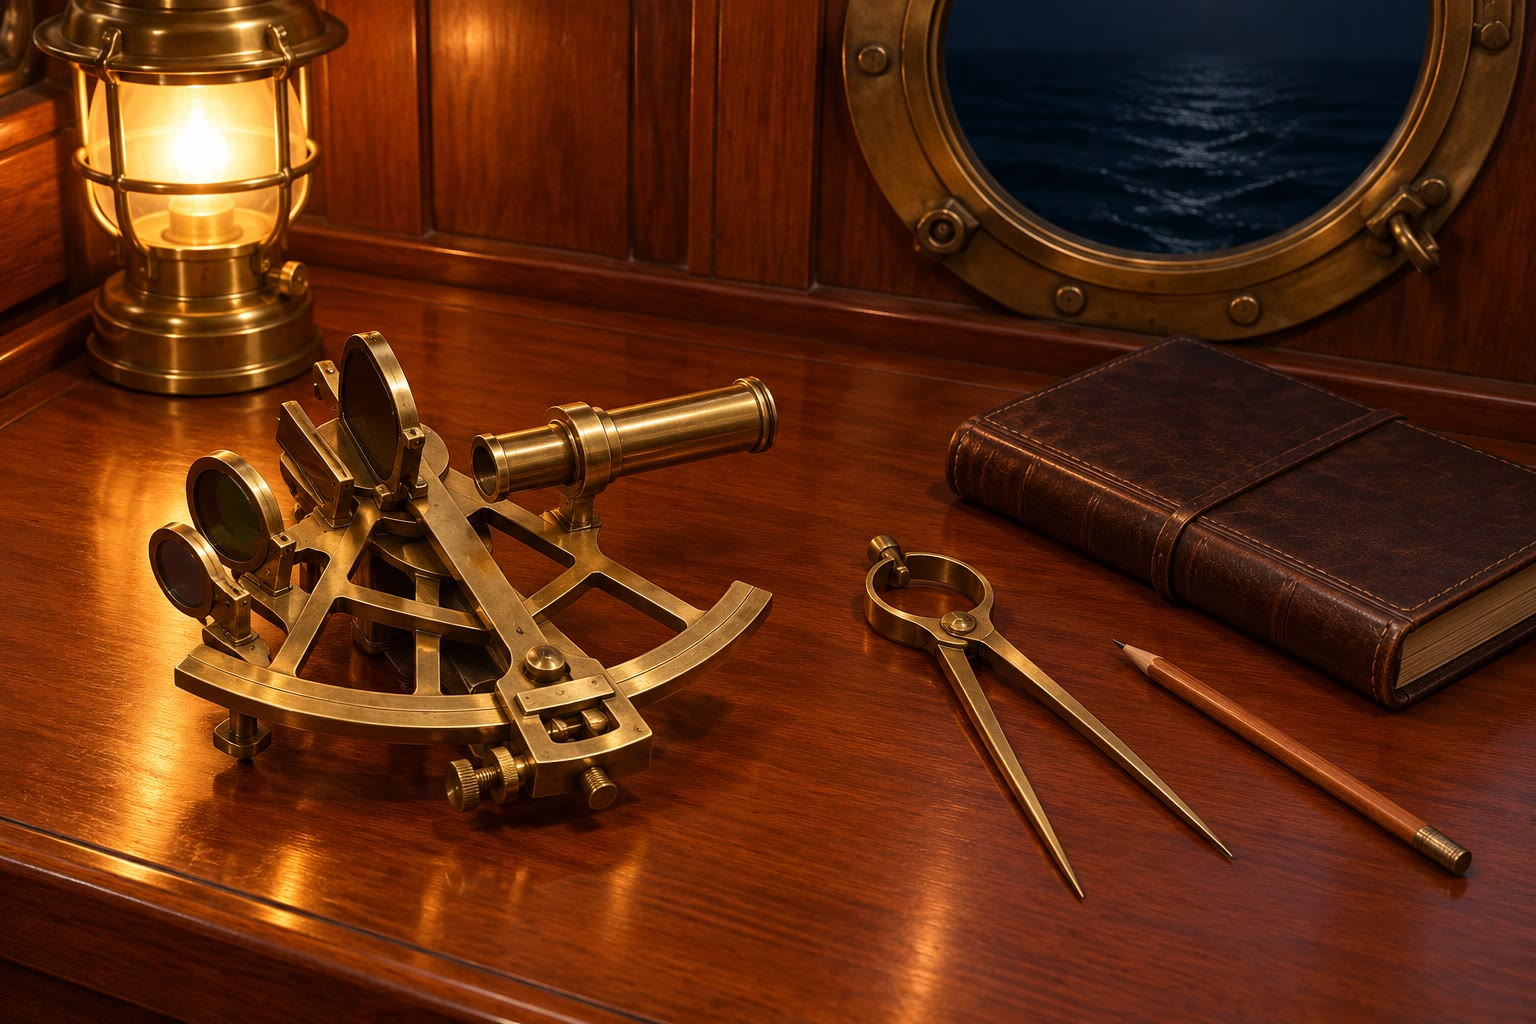
\includegraphics[width=0.55\linewidth]{images/book3/ai/b1-sextant.jpg}
\end{center}
\end{inthefield}

\section{अभ्यास}

\begin{exercise}[$\star$]\label{exo:b1:spherical-astronomy:1}
एक प्रेक्षक का \omterm{def:b1:spherical-astronomy:geographic}{अक्षांश} \ang{52} उत्तर है। उत्तरी \omterm{def:b1:spherical-astronomy:celestial-sphere}{खगोलीय ध्रुव} किस \omterm{def:b1:spherical-astronomy:horizontal}{उन्नतांश} पर है? \omterm{def:b1:spherical-astronomy:equatorial}{क्रांति} के
आधार पर कौन-से तारे वहाँ कभी अस्त नहीं होते, और कौन-से कभी उदय नहीं होते?
\end{exercise}

\begin{exercise}[$\star$]\label{exo:b1:spherical-astronomy:2}
\qty{6}{h}~\qty{45}{min} के \omterm{def:b1:spherical-astronomy:equatorial}{ऋजु आरोहण} को अंशों में बदलिए। \qty{10}{h}~\qty{0}{min} के स्थानीय
\omterm{def:b1:spherical-astronomy:sidereal-time}{नाक्षत्र काल} पर उस \omterm{def:b1:spherical-astronomy:equatorial}{ऋजु आरोहण} वाले तारे का \omterm{def:b1:spherical-astronomy:equatorial}{घंटा कोण} क्या है? क्या तारा याम्योत्तर के पूर्व
है या पश्चिम?
\end{exercise}

\begin{exercise}[$\star$]\label{exo:b1:spherical-astronomy:3}
\ang{40} उत्तरी \omterm{def:b1:spherical-astronomy:geographic}{अक्षांश} पर दोनों अयनांतों के दिन और विषुवों के दिन ($\varepsilon = \ang{23.44}$)
मध्याह्न में सूर्य का \omterm{def:b1:spherical-astronomy:horizontal}{उन्नतांश} परिकलित कीजिए।
\end{exercise}

\begin{exercise}[$\star$]\label{exo:b1:spherical-astronomy:4}
1900 अधिवर्ष था? 2000? क्या 2100 होगा? 365.2422 दिन के \omterm{def:b1:spherical-astronomy:tropical-year}{उष्णकटिबंधीय वर्ष} के सापेक्ष जूलियन
कैलेंडर प्रति शताब्दी कितने दिन खिसकता है, और ग्रेगोरी कैलेंडर कितने?
\end{exercise}

\begin{exercise}[$\star\star$]\label{exo:b1:spherical-astronomy:5}
दो बिंदु \ang{45} उत्तरी \omterm{def:b1:spherical-astronomy:geographic}{अक्षांश} पर हैं, \omterm{def:b1:spherical-astronomy:geographic}{देशांतर} \ang{0} और \ang{90} पूर्व पर। उनके बीच \omterm{def:b1:spherical-astronomy:spherical-triangle}{महावृत्त} दूरी
($R = \qty{6371}{km}$) और उनके समांतर के अनुदिश दूरी परिकलित कीजिए। कौन-सी छोटी है, और कितनी?
\end{exercise}

\begin{exercise}[$\star\star$]\label{exo:b1:spherical-astronomy:6}
\ang{48} उत्तरी \omterm{def:b1:spherical-astronomy:geographic}{अक्षांश} पर \omterm{def:b1:spherical-astronomy:equatorial}{क्रांति} \ang{20} वाले एक तारे का \omterm{def:b1:spherical-astronomy:equatorial}{घंटा कोण} \ang{30} है। उसका \omterm{def:b1:spherical-astronomy:horizontal}{उन्नतांश} और
\omterm{def:b1:spherical-astronomy:horizontal}{दिगंश} परिकलित कीजिए। प्रेक्षक को किस दिशा में देखना चाहिए?
\end{exercise}

\begin{exercise}[$\star\star$]\label{exo:b1:spherical-astronomy:7}
\ang{60} उत्तरी \omterm{def:b1:spherical-astronomy:geographic}{अक्षांश} पर जून अयनांत के दिन दिन की लंबाई परिकलित कीजिए, सूर्य को ज्यामितीय क्षितिज
पर एक बिंदु मानते हुए। दिन की लंबाई वाले चित्र पर अपने उत्तर की जाँच कीजिए।
\end{exercise}

\begin{exercise}[$\star\star$]\label{exo:b1:spherical-astronomy:8}
एक तारा आज रात स्थानीय माध्य समय 22:00 पर याम्योत्तर पार करता है। 30 दिन बाद वह किस समय
याम्योत्तर पार करेगा? कितने दिन बाद वह दोपहर में पार करेगा, जब दिन के उजाले में वह अदृश्य होगा?
\end{exercise}

\begin{exercise}[$\star\star$]\label{exo:b1:spherical-astronomy:9}
\ang{45} उत्तरी \omterm{def:b1:spherical-astronomy:geographic}{अक्षांश} पर वायुमंडल के ऊपर दोपहर के \omterm{def:b1:spherical-astronomy:insolation}{सूर्यातप} की गणना कीजिए (क) एक विषुव पर, $r = a$
मानते हुए; (ख) जून अयनांत पर, $r$ के लिए अपसौर दूरी लेते हुए। आँकड़े: $S_0 = \qty{1361}{W.m^{-2}}$,
$a = \qty{149.598e6}{km}$, अपसौर \qty{152.100e6}{km}।
\end{exercise}

\begin{exercise}[$\star\star\star$]\label{exo:b1:spherical-astronomy:10}
\cref{prop:b1:spherical-astronomy:sun-declination} का उपयोग करके, जब सूर्य का क्रांतिवृत्तीय
\omterm{def:b1:spherical-astronomy:geographic}{देशांतर} \ang{60} हो, तब सूर्य की \omterm{def:b1:spherical-astronomy:equatorial}{क्रांति} और \omterm{def:b1:spherical-astronomy:equatorial}{ऋजु आरोहण} परिकलित कीजिए। \omterm{def:b1:spherical-astronomy:equatorial}{ऋजु आरोहण} \omterm{def:b1:spherical-astronomy:geographic}{देशांतर} से कितने
अंश पीछे है? इस परिणाम से समझाइए कि \omterm{def:b1:spherical-astronomy:ecliptic}{क्रांतिवृत्त} का झुकाव समय के समीकरण में क्यों योगदान देता है।
\end{exercise}

\begin{exercise}[$\star\star\star$]\label{exo:b1:spherical-astronomy:11}
दिखाइए कि जून अयनांत पर सूर्य \omterm{def:b1:spherical-astronomy:horizontal}{दिगंश} $\mathrm{A}_0$ पर उगता है, जहाँ
$\cos\mathrm{A}_0 = \sin\varepsilon/\cos\varphi$। किस \omterm{def:b1:spherical-astronomy:geographic}{अक्षांश} पर वह ठीक उत्तर-पूर्व में उगता है?
$\ang{90} - \varepsilon$ से ऊपर के अक्षांशों पर सूत्र का क्या होता है?
\end{exercise}

\begin{exercise}[$\star\star\star$]\label{exo:b1:spherical-astronomy:12}
एक लून गोले का वह भाग है जो परस्पर विपरीत दो बिंदुओं को जोड़ने वाले दो अर्ध-महावृत्तों के बीच
पड़ता है, और ये अर्ध-महावृत्त एक-दूसरे से कोण $\theta$ पर हैं। (क) दिखाइए कि उसका क्षेत्रफल
$2\theta R^2$ है। (ख) \omterm{def:b1:spherical-astronomy:spherical-triangle}{गोलीय त्रिभुज} $ABC$ की हर भुजा को पूरे \omterm{def:b1:spherical-astronomy:spherical-triangle}{महावृत्त} तक बढ़ाने पर, दूसरी भुजाओं
के साथ मिलकर कोणों $A$, $B$, $C$ वाले लूनों के तीन विपरीत जोड़े मिलते हैं, जो गोले को ढकते हैं;
त्रिभुज और उसका विपरीत भाग तीन बार ढके जाते हैं। इससे गिरार्ड प्रमेय निकालिए: त्रिभुज का
क्षेत्रफल $R^2(A + B + C - \pi)$ है। (ग) इसे तीन समकोण वाले त्रिभुज पर, और इस अध्याय में बनाए
गए त्रिभुज (कोण \ang{89.9}, \ang{64.9}, \ang{67.4}) पर लागू कीजिए।
\end{exercise}

\section{समस्या: एक पर्वतीय वेधशाला की रात}

\begin{problem}[{सप्ताहांत समस्या --- पैरानाल वेधशाला कहाँ है, उसका आकाश क्या दिखाता है, और उसकी
सबसे लंबी रात कितनी लंबी है}]
\label{pb:b1:spherical-astronomy:1}
% ledger: mpc:paranal, mpc:greenwich, simbad:sirius, simbad:canopus, usno:seasons-2026, earth:obliquity, usno:tropical-year
% numbers computed in the scratch calculator calc/ch01.py from the rounded data
पैरानाल वेधशाला अटाकामा मरुस्थल में \omterm{def:b1:spherical-astronomy:geographic}{अक्षांश} \ang{24.63} दक्षिण और \omterm{def:b1:spherical-astronomy:geographic}{देशांतर} \ang{70.40} पश्चिम पर है।
ग्रीनविच की रॉयल वेधशाला, जिससे \omterm{def:b1:spherical-astronomy:geographic}{देशांतर} गिने जाते हैं, \ang{51.48} उत्तर और \ang{0.00} पर है।
दक्षिणी आकाश के दो चमकीले तारों के निर्देशांक ये हैं:
\begin{center}
\small
\begin{tabular}{lcc}
\hline
तारा & \omterm{def:b1:spherical-astronomy:equatorial}{ऋजु आरोहण} & \omterm{def:b1:spherical-astronomy:equatorial}{क्रांति} \\
\hline
सिरियस & \qty{6}{h}~\qty{45}{min}~\qty{9}{s} & \ang{-16.72} \\
कैनोपस & \qty{6}{h}~\qty{23}{min}~\qty{57}{s} & \ang{-52.70} \\
\hline
\end{tabular}
\end{center}
इनमें $R = \qty{6371}{km}$, $\varepsilon = \ang{23.44}$, 365.2422 दिन का \omterm{def:b1:spherical-astronomy:tropical-year}{उष्णकटिबंधीय वर्ष} लीजिए,
और सूर्य को ज्यामितीय क्षितिज पर एक बिंदु मानिए।

\medskip
\noindent\textbf{भाग I --- ग्लोब पर पैरानाल।}
\begin{enumerate}
  \item पैरानाल और ग्रीनविच के \omterm{def:b1:spherical-astronomy:geographic}{सह-अक्षांश}, तथा उनका देशांतर-अंतर दीजिए।
  \item उत्तरी ध्रुव--पैरानाल--ग्रीनविच त्रिभुज के लिए कोज्या नियम लिखिए, और दोनों वेधशालाओं के
        बीच कोणीय दूरी $\Delta$ की कोज्या परिकलित कीजिए।
  \item $\Delta$ को अंशों में और \omterm{def:b1:spherical-astronomy:spherical-triangle}{महावृत्त} दूरी को किलोमीटर में निकालिए।
  \item पैरानाल से ग्रीनविच की ओर आरंभिक दिशा परिकलित कीजिए
        (\cref{met:b1:spherical-astronomy:great-circle})।
  \item साइन नियम से दिशा की जाँच कीजिए।
  \item क्या कोई विमान, जो पूरे रास्ते यही दिशा बनाए रखे, ग्रीनविच तक पहुँचेगा? समझाइए।
\end{enumerate}

\medskip
\noindent\textbf{भाग II --- पैरानाल का आकाश।}
\begin{enumerate}[resume]
  \item पैरानाल के दक्षिणी क्षितिज के ऊपर दक्षिण \omterm{def:b1:spherical-astronomy:celestial-sphere}{खगोलीय ध्रुव} किस \omterm{def:b1:spherical-astronomy:horizontal}{उन्नतांश} पर है?
  \item सिरियस किस \omterm{def:b1:spherical-astronomy:horizontal}{उन्नतांश} पर याम्योत्तर पार करता है, और \omterm{def:b1:spherical-astronomy:celestial-sphere}{खमध्य} के किस ओर?
  \item पैरानाल पर कोई तारा किस \omterm{def:b1:spherical-astronomy:equatorial}{क्रांति} से नीचे परिध्रुवीय है? क्या कैनोपस परिध्रुवीय है?
  \item कैनोपस जो सबसे ऊँचा \omterm{def:b1:spherical-astronomy:horizontal}{उन्नतांश} प्राप्त करता है, वह क्या है?
  \item वह \omterm{def:b1:spherical-astronomy:equatorial}{घंटा कोण} परिकलित कीजिए जिस पर सिरियस उगता है, और नाक्षत्र घंटों में वह क्षितिज के
        ऊपर कितनी देर रहता है।
  \item सिरियस किस \omterm{def:b1:spherical-astronomy:horizontal}{दिगंश} पर उगता है?
\end{enumerate}

\medskip
\noindent\textbf{भाग III --- घड़ियाँ।}
\begin{enumerate}[resume]
  \item जब सिरियस याम्योत्तर पार करता है, तब स्थानीय \omterm{def:b1:spherical-astronomy:sidereal-time}{नाक्षत्र काल} क्या है?
  \item नाक्षत्र दिवस की लंबाई परिकलित कीजिए, और बताइए कि किसी तारे का याम्योत्तर-पारण हर रात
        कितने मिनट पहले होता है।
  \item 20 मार्च 2026 के मार्च विषुव पर, जब सूर्य \omterm{def:b1:spherical-astronomy:ecliptic}{वसंत विषुव-बिंदु} के पास होता है, स्थानीय माध्य
        मध्यरात्रि पर स्थानीय \omterm{def:b1:spherical-astronomy:sidereal-time}{नाक्षत्र काल} \qty{12}{h} लीजिए; तब वह हर दिन $24/365.2422$ घंटे बढ़ता
        है। विषुव के कितने दिन बाद सिरियस स्थानीय माध्य मध्यरात्रि पर याम्योत्तर पार करता है?
        किस तिथि को?
  \item उस रात पैरानाल का स्थानीय माध्य समय ग्रीनविच के समय से कितना भिन्न है?
  \item \omterm{def:b1:spherical-astronomy:solar-time}{समय का समीकरण} तब लगभग \qty{-3}{min} है। जब सिरियस याम्योत्तर पार करता है, तब वेधशाला की
        धूपघड़ी कौन-सा समय (\omterm{def:b1:spherical-astronomy:solar-time}{स्पष्ट सौर काल}) दिखाती है?
  \item एक सप्ताह बाद वह कितने पहले पार करता है?
\end{enumerate}

\medskip
\noindent\textbf{भाग IV --- सबसे लंबी रात।}
\begin{enumerate}[resume]
  \item हर अयनांत पर सूर्य की \omterm{def:b1:spherical-astronomy:equatorial}{क्रांति} क्या है?
  \item जून और दिसंबर अयनांतों पर पैरानाल में मध्याह्न में सूर्य का \omterm{def:b1:spherical-astronomy:horizontal}{उन्नतांश} परिकलित कीजिए। दिसंबर
        में वह \omterm{def:b1:spherical-astronomy:celestial-sphere}{खमध्य} के किस ओर है?
  \item दिसंबर अयनांत पर सूर्य-पृथ्वी दूरी माध्य दूरी की 0.9837 गुना है। पैरानाल के ऊपर, वायुमंडल
        के ऊपर, मध्याह्न के \omterm{def:b1:spherical-astronomy:insolation}{सूर्यातप} की गणना कीजिए ($S_0 = \qty{1361}{W.m^{-2}}$)।
  \item पैरानाल पर किस अयनांत पर रात सबसे लंबी है? उस तिथि पर सूर्यास्त का \omterm{def:b1:spherical-astronomy:equatorial}{घंटा कोण} परिकलित कीजिए।
  \item उस तिथि पर सूर्य किस \omterm{def:b1:spherical-astronomy:horizontal}{दिगंश} पर उगता है?
  \item पैरानाल पर वर्ष की सबसे लंबी रात की अवधि घंटों और मिनटों में निकालिए।
\end{enumerate}
\end{problem}
